\documentclass[11pt,a4paper]{article}

\usepackage[utf8]{inputenc}
\usepackage[margin=0.9in]{geometry}
\usepackage[T1]{fontenc}
\usepackage{lmodern}
\usepackage{amsmath,amssymb,amsfonts,amsthm}
\usepackage{booktabs}
\usepackage{graphicx}
\usepackage[protrusion=true,expansion=false]{microtype}
\usepackage{tikz}
\usetikzlibrary{shapes,arrows.meta,positioning,fit,calc,backgrounds,decorations.pathreplacing}
\usepackage{tcolorbox}
\tcbuselibrary{skins,breakable}
\usepackage{hyperref}
\usepackage{xcolor}
\usepackage{listings}
\usepackage{enumitem}

% Color Palette
\definecolor{navyblue}{RGB}{12,44,95}
\definecolor{deepteal}{RGB}{10,80,95}
\definecolor{crimson}{RGB}{160,25,35}
\definecolor{amber}{RGB}{200,120,20}
\definecolor{softblue}{RGB}{235,242,250}
\definecolor{softgreen}{RGB}{235,247,238}
\definecolor{softyellow}{RGB}{254,249,235}
\definecolor{darkgray}{RGB}{50,50,50}
\definecolor{codebg}{RGB}{248,249,251}

\hypersetup{
    colorlinks=true,
    linkcolor=navyblue,
    citecolor=navyblue,
    urlcolor=navyblue
}

\newtheorem{theorem}{Theorem}[section]
\newtheorem{lemma}[theorem]{Lemma}
\newtheorem{definition}[theorem]{Definition}

% Custom TColorBoxes for Bachelor-Level Pedagogy
\newtcolorbox{intuitionbox}[1][]{
    enhanced,
    breakable,
    colback=softblue,
    colframe=navyblue,
    arc=3mm,
    boxrule=1.2pt,
    title={\textbf{\large [Intuition \& Analogy] #1}},
    coltitle=white,
    colbacktitle=navyblue,
    fonttitle=\bfseries,
    attach boxed title to top left={yshift=-2mm,xshift=4mm},
    boxed title style={arc=1.5mm},
    top=4mm,bottom=3mm,left=4mm,right=4mm
}

\newtcolorbox{mathcheck}[1][]{
    enhanced,
    breakable,
    colback=softgreen,
    colframe=forestgreen!80!black,
    arc=3mm,
    boxrule=1.2pt,
    title={\textbf{\large [Math \& Dimension Breakdown] #1}},
    coltitle=white,
    colbacktitle=forestgreen!80!black,
    fonttitle=\bfseries,
    attach boxed title to top left={yshift=-2mm,xshift=4mm},
    boxed title style={arc=1.5mm},
    top=4mm,bottom=3mm,left=4mm,right=4mm
}

\newtcolorbox{codebox}[1][]{
    enhanced,
    breakable,
    colback=codebg,
    colframe=darkgray!70,
    arc=2mm,
    boxrule=1pt,
    title={\textbf{\texttt{PyTorch} Implementation Link: #1}},
    coltitle=white,
    colbacktitle=darkgray!80,
    fonttitle=\small\ttfamily,
    attach boxed title to top left={yshift=-2mm,xshift=4mm},
    boxed title style={arc=1mm},
    top=3mm,bottom=2mm,left=3mm,right=3mm
}

\newtcolorbox{warningbox}[1][]{
    enhanced,
    breakable,
    colback=softyellow,
    colframe=amber!90!black,
    arc=3mm,
    boxrule=1.2pt,
    title={\textbf{\large [Systems Engineering Note] #1}},
    coltitle=white,
    colbacktitle=amber!90!black,
    fonttitle=\bfseries,
    attach boxed title to top left={yshift=-2mm,xshift=4mm},
    boxed title style={arc=1.5mm},
    top=4mm,bottom=3mm,left=4mm,right=4mm
}

\definecolor{forestgreen}{RGB}{34,139,34}

% Listings formatting for PyTorch code
\lstset{
    language=Python,
    backgroundcolor=\color{codebg},
    basicstyle=\footnotesize\ttfamily,
    keywordstyle=\color{navyblue}\bfseries,
    commentstyle=\color{gray}\itshape,
    stringstyle=\color{crimson},
    numbers=left,
    numberstyle=\tiny\color{gray},
    numbersep=7pt,
    frame=single,
    framerule=0.5pt,
    rulecolor=\color{gray!40},
    breaklines=true,
    showstringspaces=false
}

\title{\LARGE \textbf{Demystifying the Temporal Fusion Transformer (TFT)}\\
\Large \textbf{A Bachelor's Guide to Architecture, Mathematics, and Real-Time Ad Pacing}}
\author{\textbf{Autonomous AI Systems Research Group} \\
Repository Guide: \texttt{TFT\_Ad\_pacing} \quad | \quad Target: ICIIT 2027 (ACM ICPS)}
\date{September 2026}

\begin{document}

\maketitle

\begin{abstract}
This guide is written specifically for undergraduate students in Computer Science, Data Science, and Software Engineering. Deep learning research papers often introduce complex neural network architectures using dense mathematical symbols without providing the underlying operational intuition. Here, we unpack the \textbf{Temporal Fusion Transformer (TFT)} for programmatic ad spend pacing from first principles. We explain every equation using familiar concepts: basic linear algebra (matrix multiplications, vector projections), single-variable calculus (gradients and backpropagation), and standard PyTorch tensor manipulations. We explore why standard Transformers fail on time series, how Gated Linear Units (GLU) act like digital transistors, why Variable Selection Networks (VSN) filter noise, how Interpretable Multi-Head Attention enables real-world explainability, and why Apple Silicon Metal Performance Shaders (MPS) crashed with a $1,376,256$-byte memory error.
\end{abstract}

\tableofcontents
\newpage

\section{Introduction: The Real-World Engineering Problem}

\subsection{What is Programmatic Ad Pacing?}
Imagine you are managing an advertising budget of \$10,000 for a 7-day marketing campaign ($T = 168\text{ hours}$). Every millisecond, mobile phones and web browsers load ad slots. An automated ad exchange holds an auction to decide which ad to show. Your system—the \textbf{Demand-Side Platform (DSP)}—must submit a dollar bid $b_t$ for each auction.

\begin{intuitionbox}[The Golden Rule of Pacing]
If you bid full price on every single impression starting at midnight:
\begin{itemize}
    \item You will win every auction in the middle of the night when most people are asleep and low-value bots are browsing.
    \item Your entire \$10,000 budget will be \textbf{exhausted by 4:00 AM on Day 1}.
    \item You will have \$0 remaining for prime-time hours (7:00 PM - 10:00 PM) when active, high-intent human shoppers are online.
\end{itemize}
This catastrophic failure is called \textbf{Premature Budget Depletion}.
\end{intuitionbox}

To solve this, ad systems introduce a \textbf{pacing multiplier} $\alpha_t \in [0.05, 1.0]$. The DSP evaluates the intrinsic value of an ad slot $v(x)$ (e.g., \$2.00) and scales the outgoing bid:
\begin{equation}
    b_t(x) = \alpha_t \cdot v(x)
\end{equation}
\begin{itemize}
    \item When $\alpha_t = 1.0$, the system bids aggressively.
    \item When $\alpha_t = 0.10$, the system throttles back, entering only the highest-conviction auctions.
\end{itemize}
Our goal is to compute the optimal $\alpha_t$ at every discrete hour $t \in \{1, 2, \dots, T\}$ so that the campaign spends its budget smoothly and effectively across all 168 hours without ever running out of money early.

\subsection{Why Simple Methods Fail}
Why can't we just divide the budget evenly? E.g., $\text{Hourly Target} = \frac{\$10,000}{168\text{ hours}} = \$59.52/\text{hour}$?
\begin{enumerate}
    \item \textbf{Circadian Rhythms (Day vs. Night):} At 3:00 AM, there is very little Internet traffic. Even if you bid aggressively, you might only be able to spend \$15. At 8:00 PM, traffic surges tenfold. A rigid uniform target forces the system to choke during peak hours and fail to deliver during slow hours.
    \item \textbf{Auction Competitor Volatility:} Competitors suddenly start or pause their own campaigns, causing market clearing prices to spike unpredictably.
    \item \textbf{Deterministic Seasonality vs. Stochastic Noise:} While we know for sure when Saturday arrives (calendar feature), we cannot know the exact winning price without probabilistic forecasting.
\end{enumerate}

This requires a deep learning architecture that can simultaneously handle:
\begin{itemize}
    \item \textbf{Static metadata:} Total campaign budget $B$, duration $T$.
    \item \textbf{Observed past data:} Hourly spend history, win rates, historical CPM.
    \item \textbf{Known future data:} Day of week, hour of day, weekend indicators.
\end{itemize}
That model is the \textbf{Temporal Fusion Transformer (TFT)}.

---

\section{High-Level Architecture Overview}

Before diving into the equations, let us look at the complete architectural pipeline shown in Figure~\ref{fig:tft_student_flow}.

\begin{figure*}[htbp]
\centering
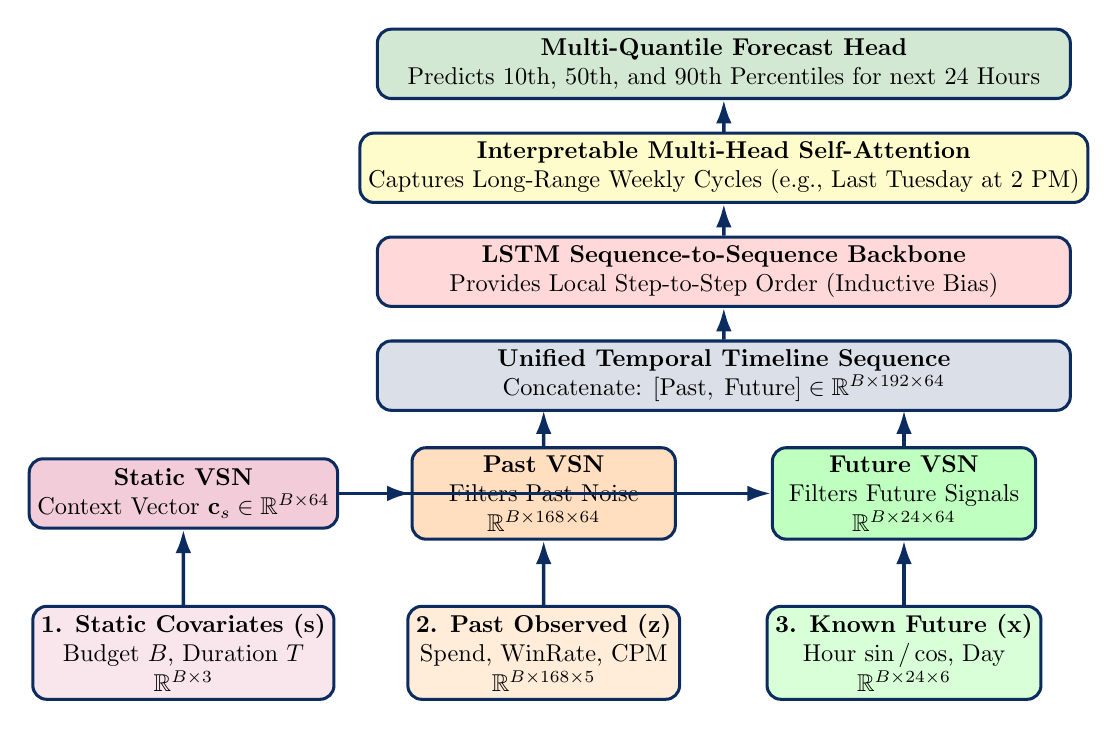
\begin{tikzpicture}[
    scale=0.88, every node/.style={transform shape},
    box/.style={rectangle, draw=navyblue, fill=softblue, rounded corners=5pt, line width=1.1pt, minimum width=3.8cm, minimum height=1cm, align=center},
    flow/.style={-{Latex[length=3mm, width=2mm]}, line width=1.3pt, color=navyblue},
    annot/.style={font=\footnotesize\itshape, text=darkgray}
]

% Inputs
\node[box, fill=purple!10] (static) at (0, 0) {\textbf{1. Static Covariates ($\mathbf{s}$)}\\Budget $B$, Duration $T$\\$\mathbb{R}^{B \times 3}$};
\node[box, fill=orange!15] (past) at (5.2, 0) {\textbf{2. Past Observed ($\mathbf{z}$)}\\Spend, WinRate, CPM\\$\mathbb{R}^{B \times 168 \times 5}$};
\node[box, fill=green!15] (future) at (10.4, 0) {\textbf{3. Known Future ($\mathbf{x}$)}\\Hour $\sin/\cos$, Day\\$\mathbb{R}^{B \times 24 \times 6}$};

% VSN
\node[box, fill=purple!20] (vsn_s) at (0, 2.3) {\textbf{Static VSN}\\Context Vector $\mathbf{c}_s \in \mathbb{R}^{B \times 64}$};
\node[box, fill=orange!25] (vsn_p) at (5.2, 2.3) {\textbf{Past VSN}\\Filters Past Noise\\$\mathbb{R}^{B \times 168 \times 64}$};
\node[box, fill=green!25] (vsn_f) at (10.4, 2.3) {\textbf{Future VSN}\\Filters Future Signals\\$\mathbb{R}^{B \times 24 \times 64}$};

% Unified Sequence
\node[box, fill=navyblue!15, minimum width=10cm] (seq) at (7.8, 4.0) {\textbf{Unified Temporal Timeline Sequence}\\Concatenate: $[\text{Past}, \; \text{Future}] \in \mathbb{R}^{B \times 192 \times 64}$};

% LSTM
\node[box, fill=red!15, minimum width=10cm] (lstm) at (7.8, 5.5) {\textbf{LSTM Sequence-to-Sequence Backbone}\\Provides Local Step-to-Step Order (Inductive Bias)};

% Attention
\node[box, fill=yellow!20, minimum width=10cm] (attn) at (7.8, 7.0) {\textbf{Interpretable Multi-Head Self-Attention}\\Captures Long-Range Weekly Cycles (e.g., Last Tuesday at 2 PM)};

% Output Head
\node[box, fill=forestgreen!20, minimum width=10cm] (out) at (7.8, 8.5) {\textbf{Multi-Quantile Forecast Head}\\Predicts 10th, 50th, and 90th Percentiles for next 24 Hours};

% Arrows
\draw[flow] (static) -- (vsn_s);
\draw[flow] (past) -- (vsn_p);
\draw[flow] (future) -- (vsn_f);

\draw[flow] (vsn_s.east) -- (vsn_p.west);
\draw[flow] (vsn_s.east) -- ++(0.5,0) |- (vsn_f.west);

\draw[flow] (vsn_p) -- (5.2, 3.5);
\draw[flow] (vsn_f) -- (10.4, 3.5);

\draw[flow] (seq) -- (lstm);
\draw[flow] (lstm) -- (attn);
\draw[flow] (attn) -- (out);

\end{tikzpicture}
\caption{Dataflow through the Temporal Fusion Transformer. Dimensions correspond to Mini-Batch size $B=32$, Lookback $k=168\text{h}$, Forecast Horizon $\tau=24\text{h}$, and Latent Dimension $d=64$.}
\label{fig:tft_student_flow}
\end{figure*}

\subsection{The Three Input Streams}
At every discrete step $t$, the model receives three distinct types of inputs:
\begin{enumerate}
    \item \textbf{Static Metadata ($\mathbf{s} \in \mathbb{R}^3$):} Features that never change during the campaign:
    \begin{itemize}
        \item Total budget $B$ (e.g., \$10,000)
        \item Nominal hourly velocity $B/T$ (e.g., \$59.52/hour)
        \item Total campaign duration $T$ (168 hours)
    \end{itemize}
    \item \textbf{Observed Past Inputs ($\mathbf{z}_\tau \in \mathbb{R}^5$ for $\tau \in [t-167, t]$):} Historical facts logged over the past 7 days (168 hours):
    \begin{itemize}
        \item Realized hourly spend $y_\tau$
        \item Winning auction impressions $I_\tau$
        \item Empirical auction win rate $w_\tau \in [0, 1]$
        \item Effective cost-per-mille $\text{CPM}_\tau$
        \item Budget consumption ratio $S_\tau / B$
    \end{itemize}
    \item \textbf{Known Future Inputs ($\mathbf{x}_{t+\tau} \in \mathbb{R}^6$ for $\tau \in [1, 24]$):} Features we know in advance about the upcoming 24 hours:
    \begin{itemize}
        \item Cyclical hour of day: $\sin(2\pi h / 24)$ and $\cos(2\pi h / 24)$
        \item Cyclical day of week: $\sin(2\pi d / 7)$ and $\cos(2\pi d / 7)$
        \item Weekend binary flag: $\mathbb{I}_{\text{weekend}} \in \{0, 1\}$
        \item Remaining time fraction: $(T - (t+\tau)) / T$
    \end{itemize}
\end{enumerate}

---

\section{The Core Building Blocks: From Transistors to Neural Gates}

Standard deep neural networks are built by stacking linear transformations ($\mathbf{W}\mathbf{x} + \mathbf{b}$) and fixed non-linearities like $\text{ReLU}(z) = \max(0, z)$. However, real-time ad markets suffer from extreme regime changes. For instance, an equation that is useful during midday trading might be completely useless (or harmful) at 3:00 AM. 

To solve this, TFT introduces two fundamental mathematical components:
\begin{enumerate}
    \item The \textbf{Gated Linear Unit (GLU)}
    \item The \textbf{Gated Residual Network (GRN)}
\end{enumerate}

\subsection{Gated Linear Unit (GLU): The Neural Transistor}

\begin{intuitionbox}[The Digital Transistor Analogy]
In computer hardware, a transistor uses a control voltage on a `gate' pin to decide whether electric current flows or is stopped completely.
A \textbf{Gated Linear Unit (GLU)} does the exact same thing for numbers inside a neural network:
\begin{itemize}
    \item One path calculates candidate information $\mathbf{v}$ (what the network might want to say).
    \item The second path calculates a gate signal $\mathbf{g} \in [0, 1]$ using a Sigmoid function (how much of that information should be allowed through).
    \item When $\mathbf{g} \approx 0$, the gate is closed, blocking the signal. When $\mathbf{g} \approx 1$, the gate is open.
\end{itemize}
\end{intuitionbox}

\begin{figure}[htbp]
\centering
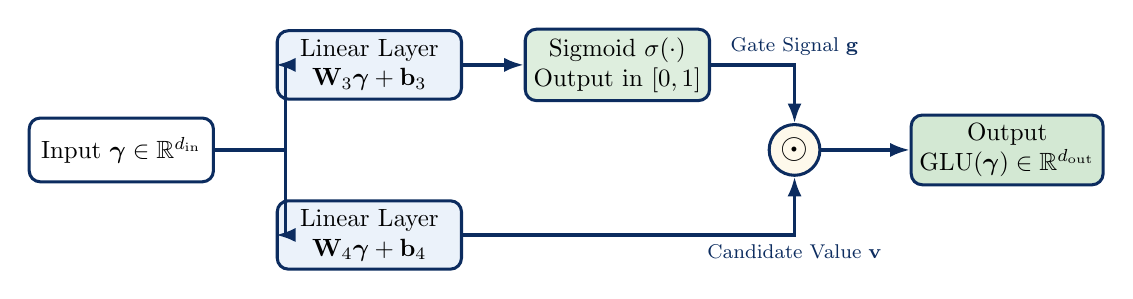
\begin{tikzpicture}[
    scale=0.9, every node/.style={transform shape},
    box/.style={rectangle, draw=navyblue, fill=softblue, rounded corners=4pt, line width=1.1pt, minimum width=2.6cm, minimum height=0.9cm, align=center},
    op/.style={circle, draw=navyblue, fill=softyellow, line width=1.1pt, inner sep=2pt},
    flow/.style={-{Latex[length=2.5mm, width=1.8mm]}, line width=1.2pt, color=navyblue}
]

\node[box, fill=white] (in) at (0, 0) {Input $\boldsymbol{\gamma} \in \mathbb{R}^{d_{\text{in}}}$};

\node[box] (lin1) at (3.5, 1.2) {Linear Layer\\$\mathbf{W}_3 \boldsymbol{\gamma} + \mathbf{b}_3$};
\node[box] (lin2) at (3.5, -1.2) {Linear Layer\\$\mathbf{W}_4 \boldsymbol{\gamma} + \mathbf{b}_4$};

\node[box, fill=forestgreen!15] (sig) at (7.0, 1.2) {Sigmoid $\sigma(\cdot)$\\Output in $[0, 1]$};

\node[op] (mult) at (9.5, 0) {\Large $\odot$};

\node[box, fill=forestgreen!20] (out) at (12.5, 0) {Output\\$\mathrm{GLU}(\boldsymbol{\gamma}) \in \mathbb{R}^{d_{\text{out}}}$};

\draw[flow] (in.east) -- ++(1,0) |- (lin1.west);
\draw[flow] (in.east) -- ++(1,0) |- (lin2.west);

\draw[flow] (lin1) -- (sig);
\draw[flow] (sig.east) -| (mult.north) node[midway, above, font=\footnotesize] {Gate Signal $\mathbf{g}$};
\draw[flow] (lin2.east) -| (mult.south) node[midway, below, font=\footnotesize] {Candidate Value $\mathbf{v}$};

\draw[flow] (mult) -- (out);

\end{tikzpicture}
\caption{Architectural dataflow inside a Gated Linear Unit (GLU). The $\odot$ symbol represents the element-wise Hadamard product.}
\label{fig:glu_diagram}
\end{figure}

Mathematically, for an input vector $\boldsymbol{\gamma} \in \mathbb{R}^{d_{\text{in}}}$:
\begin{equation}
    \mathrm{GLU}(\boldsymbol{\gamma}) = \sigma\left(\mathbf{W}_3 \boldsymbol{\gamma} + \mathbf{b}_3\right) \odot \left(\mathbf{W}_4 \boldsymbol{\gamma} + \mathbf{b}_4\right)
\end{equation}
where:
\begin{itemize}
    \item $\mathbf{W}_3, \mathbf{W}_4 \in \mathbb{R}^{d_{\text{out}} \times d_{\text{in}}}$ are learnable weight matrices.
    \item $\mathbf{b}_3, \mathbf{b}_4 \in \mathbb{R}^{d_{\text{out}}}$ are bias vectors.
    \item $\sigma(z) = \frac{1}{1 + e^{-z}}$ is the element-wise sigmoid function mapping values to $(0, 1)$.
    \item $\odot$ denotes the \textbf{Hadamard product} (element-by-element multiplication).
\end{itemize}

\begin{mathcheck}[Linear Algebra of Hadamard Product vs Matrix Multiplication]
Recall from linear algebra:
\begin{itemize}
    \item Standard matrix multiplication $\mathbf{A} \mathbf{x}$ combines elements across columns: $(\mathbf{A}\mathbf{x})_i = \sum_j A_{ij} x_j$.
    \item In contrast, the Hadamard product $\mathbf{u} \odot \mathbf{v}$ operates on vectors of the \textit{exact same size}:
    \begin{equation}
        \begin{bmatrix} u_1 \\ u_2 \\ \vdots \\ u_d \end{bmatrix} \odot \begin{bmatrix} v_1 \\ v_2 \\ \vdots \\ v_d \end{bmatrix} = \begin{bmatrix} u_1 \cdot v_1 \\ u_2 \cdot v_2 \\ \vdots \\ u_d \cdot v_d \end{bmatrix}
    \end{equation}
    If $u_1 = 0.01$ (gate closed) and $v_1 = 85.4$, their product is $0.854 \approx 0$. If $u_2 = 0.99$ (gate open) and $v_2 = 42.0$, their product is $41.58 \approx 42.0$.
\end{itemize}
\end{mathcheck}

\begin{codebox}[Direct Code from \texttt{pipeline/models/tft\_model.py}]
\begin{lstlisting}
class GLU(nn.Module):
    def __init__(self, input_dim: int, output_dim: int):
        super().__init__()
        # Project once into twice the output dimension: [values, gates]
        self.fc = nn.Linear(input_dim, output_dim * 2)

    def forward(self, x: torch.Tensor) -> torch.Tensor:
        val, gate = self.fc(x).chunk(2, dim=-1)
        return val * torch.sigmoid(gate)
\end{lstlisting}
\end{codebox}

---

\subsection{Gated Residual Network (GRN): The Fundamental Non-Linear Atom}

A standard problem with deep neural networks is that if you stack too many layers, early layers can over-process simple data, or gradients can vanish during backpropagation. 

The \textbf{Gated Residual Network (GRN)} solves this by combining four elements:
\begin{enumerate}
    \item \textbf{Dense Transformations with ELU activation}: To extract rich features when needed.
    \item \textbf{Context Conditioning}: To allow external information (e.g., static campaign budget) to steer the transformation.
    \item \textbf{GLU Gating}: To close the gate if non-linear processing is unhelpful.
    \item \textbf{Skip Connection (Residual) + Layer Normalization}: So the network can act as an identity pass-through.
\end{enumerate}

\begin{figure}[htbp]
\centering
\resizebox{\linewidth}{!}{%
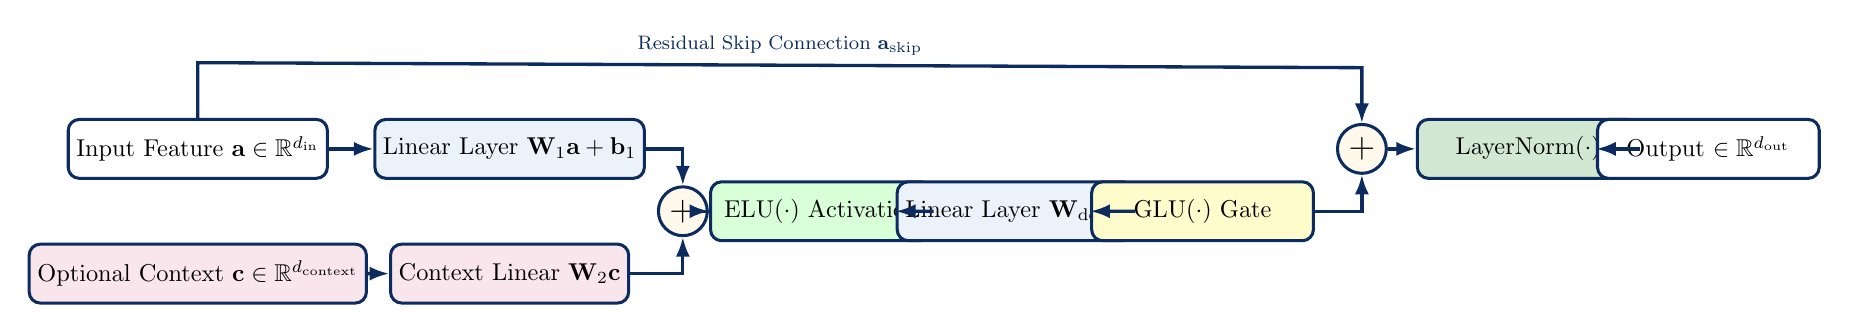
\begin{tikzpicture}[
    scale=0.88, every node/.style={transform shape},
    box/.style={rectangle, draw=navyblue, fill=softblue, rounded corners=4pt, line width=1.1pt, minimum width=3.2cm, minimum height=0.85cm, align=center},
    op/.style={circle, draw=navyblue, fill=softyellow, line width=1.1pt, inner sep=2pt},
    flow/.style={-{Latex[length=2.5mm, width=1.8mm]}, line width=1.2pt, color=navyblue}
]

\node[box, fill=white] (x) at (0, 0) {Input Feature $\mathbf{a} \in \mathbb{R}^{d_{\text{in}}}$};
\node[box, fill=purple!10] (c) at (0, -1.8) {Optional Context $\mathbf{c} \in \mathbb{R}^{d_{\text{context}}}$};

\node[box] (dense1) at (4.5, 0) {Linear Layer $\mathbf{W}_1 \mathbf{a} + \mathbf{b}_1$};
\node[box, fill=purple!10] (dense_c) at (4.5, -1.8) {Context Linear $\mathbf{W}_2 \mathbf{c}$};

\node[op] (add1) at (7.0, -0.9) {\Large $+$};
\node[box, fill=green!15] (elu) at (9.0, -0.9) {$\text{ELU}(\cdot)$ Activation};
\node[box] (dense2) at (11.8, -0.9) {Linear Layer $\mathbf{W}_{\text{dense}}$};
\node[box, fill=yellow!20] (glu) at (14.5, -0.9) {$\mathrm{GLU}(\cdot)$ Gate};

\node[op] (add2) at (16.8, 0) {\Large $+$};
\node[box, fill=forestgreen!20] (norm) at (19.2, 0) {$\mathrm{LayerNorm}(\cdot)$};
\node[box, fill=white] (out) at (21.8, 0) {Output $\in \mathbb{R}^{d_{\text{out}}}$};

% Connect
\draw[flow] (x) -- (dense1);
\draw[flow] (c) -- (dense_c);
\draw[flow] (dense1.east) -| (add1.north);
\draw[flow] (dense_c.east) -| (add1.south);
\draw[flow] (add1) -- (elu);
\draw[flow] (elu) -- (dense2);
\draw[flow] (dense2) -- (glu);
\draw[flow] (glu.east) -| (add2.south);

% Skip Connection
\draw[flow] (x.north) -- ++(0, 0.8) -- node[above, font=\footnotesize] {Residual Skip Connection $\mathbf{a}_{\text{skip}}$} ($(add2.north) + (0, 0.8)$) -- (add2.north);

\draw[flow] (add2) -- (norm);
\draw[flow] (norm) -- (out);

\end{tikzpicture}%
}
\caption{Architectural layout of the Gated Residual Network (GRN). If the input is already optimal, the GLU gate outputs zero, and the network safely behaves as $\mathrm{LayerNorm}(\mathbf{a}_{\text{skip}})$.}
\label{fig:grn_diagram}
\end{figure}

The mathematical equations defining the GRN are:
\begin{align}
    \boldsymbol{\eta}_1 &= \mathbf{W}_1 \mathbf{a} + \mathbf{W}_2 \mathbf{c} + \mathbf{b}_1 \\
    \boldsymbol{\eta}_2 &= \mathbf{W}_{\text{dense}} \left(\mathrm{ELU}(\boldsymbol{\eta}_1)\right) + \mathbf{b}_{\text{dense}} \\
    \mathbf{a}_{\text{skip}} &= \begin{cases} \mathbf{a}, & \text{if } d_{\text{in}} = d_{\text{out}} \\ \mathbf{W}_{\text{skip}} \mathbf{a}, & \text{if } d_{\text{in}} \ne d_{\text{out}} \end{cases} \\
    \mathrm{GRN}(\mathbf{a}, \mathbf{c}) &= \mathrm{LayerNorm}\left(\mathbf{a}_{\text{skip}} + \mathrm{GLU}(\boldsymbol{\eta}_2)\right)
\end{align}

\begin{intuitionbox}[Why use ELU instead of ReLU?]
The Exponential Linear Unit ($\mathrm{ELU}$) is defined as:
\begin{equation}
    \mathrm{ELU}(z) = \begin{cases} z, & z > 0 \\ \alpha(e^z - 1), & z \le 0 \end{cases}
\end{equation}
Unlike standard $\mathrm{ReLU}$ which sets all negative numbers strictly to $0$ (causing the infamous `dying ReLU' problem where neurons permanently stop learning because their derivative is zero), $\mathrm{ELU}$ has a continuous non-zero derivative for negative values:
\begin{equation}
    \frac{d}{dz}\mathrm{ELU}(z) = \begin{cases} 1, & z > 0 \\ \alpha e^z, & z \le 0 \end{cases}
\end{equation}
This allows gradients to flow backwards even during extreme market dips or zero-spend periods.
\end{intuitionbox}

\begin{codebox}[Direct Code from \texttt{pipeline/models/tft\_model.py}]
\begin{lstlisting}
class GatedResidualNetwork(nn.Module):
    def __init__(self, input_dim: int, hidden_dim: int, output_dim: int, context_dim: int = None, dropout: float = 0.1):
        super().__init__()
        self.fc1 = nn.Linear(input_dim, hidden_dim)
        self.context_fc = nn.Linear(context_dim, hidden_dim, bias=False) if context_dim else None
        self.fc2 = nn.Linear(hidden_dim, hidden_dim)
        self.dropout = nn.Dropout(dropout)
        self.glu = GLU(hidden_dim, output_dim)
        self.layer_norm = nn.LayerNorm(output_dim)
        self.skip = nn.Identity() if input_dim == output_dim else nn.Linear(input_dim, output_dim)

    def forward(self, x: torch.Tensor, context: torch.Tensor = None) -> torch.Tensor:
        residual = self.skip(x)
        h = self.fc1(x)
        if context is not None and self.context_fc is not None:
            h = h + self.context_fc(context)
        h = F.elu(h)
        h = self.fc2(h)
        h = self.dropout(h)
        h = self.glu(h)
        return self.layer_norm(residual + h)
\end{lstlisting}
\end{codebox}

---

\section{Variable Selection Networks (VSN): Learning What to Ignore}

\subsection{The Problem: Noisy Features}
In ad spend pacing, we feed the model multiple historical features:
\begin{equation}
    \mathbf{z}_t = [y_t \text{ (spend)}, \; I_t \text{ (impressions)}, \; w_t \text{ (win rate)}, \; \text{CPM}_t, \; S_t/B \text{ (depletion)}]
\end{equation}
In some hours, CPM fluctuates violently due to random auction noise that has nothing to do with long-term trends. If a model treats all features equally, this noise corrupts the forecast.

\begin{intuitionbox}[The Expert Committee Analogy]
Think of the $m$ features as $m$ advisors standing in a room:
\begin{itemize}
    \item Advisor 1 shouts: ``Look at spend!''
    \item Advisor 2 shouts: ``Look at CPM!''
    \item Advisor 3 shouts: ``Look at win rate!''
\end{itemize}
The \textbf{Variable Selection Network (VSN)} acts as the intelligent Committee Chairman. Conditioned on the static campaign context (e.g., ``This is a high-budget, fast-depleting campaign''), the Chairman computes a set of \textbf{Softmax attention weights} $v_1, v_2, \dots, v_m$ that sum to $1.0$:
\begin{equation}
    v_1 + v_2 + \dots + v_m = 1.0, \quad v_j \ge 0
\end{equation}
If CPM is noisy right now, the Chairman assigns $v_{\text{CPM}} = 0.02$ and $v_{\text{spend}} = 0.78$. The model essentially turns down the microphone on noisy features!
\end{intuitionbox}

\begin{figure}[htbp]
\centering
\resizebox{\linewidth}{!}{%
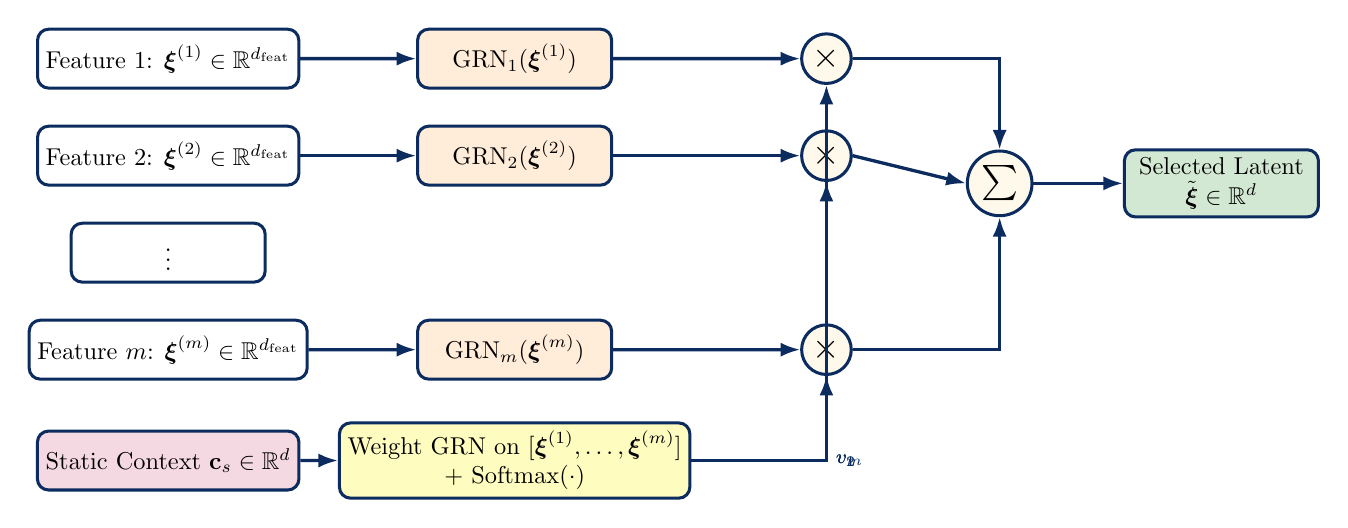
\begin{tikzpicture}[
    scale=0.88, every node/.style={transform shape},
    box/.style={rectangle, draw=navyblue, fill=softblue, rounded corners=4pt, line width=1.1pt, minimum width=2.8cm, minimum height=0.85cm, align=center},
    op/.style={circle, draw=navyblue, fill=softyellow, line width=1.1pt, inner sep=2pt},
    flow/.style={-{Latex[length=2.5mm, width=1.8mm]}, line width=1.2pt, color=navyblue}
]

% Input features
\node[box, fill=white] (f1) at (0, 1.8) {Feature 1: $\boldsymbol{\xi}^{(1)} \in \mathbb{R}^{d_{\text{feat}}}$};
\node[box, fill=white] (f2) at (0, 0.4) {Feature 2: $\boldsymbol{\xi}^{(2)} \in \mathbb{R}^{d_{\text{feat}}}$};
\node[box, fill=white] (f3) at (0, -1.0) {$\vdots$};
\node[box, fill=white] (fm) at (0, -2.4) {Feature $m$: $\boldsymbol{\xi}^{(m)} \in \mathbb{R}^{d_{\text{feat}}}$};

% Context
\node[box, fill=purple!15] (ctx) at (0, -4.0) {Static Context $\mathbf{c}_s \in \mathbb{R}^d$};

% Feature GRNs
\node[box, fill=orange!15] (grn1) at (5.0, 1.8) {$\mathrm{GRN}_1(\boldsymbol{\xi}^{(1)})$};
\node[box, fill=orange!15] (grn2) at (5.0, 0.4) {$\mathrm{GRN}_2(\boldsymbol{\xi}^{(2)})$};
\node[box, fill=orange!15] (grnm) at (5.0, -2.4) {$\mathrm{GRN}_m(\boldsymbol{\xi}^{(m)})$};

% Weight GRN
\node[box, fill=yellow!25, minimum width=4cm] (w_grn) at (5.0, -4.0) {Weight GRN on $[\boldsymbol{\xi}^{(1)}, \dots, \boldsymbol{\xi}^{(m)}]$\\+ $\mathrm{Softmax}(\cdot)$};

% Weight outputs
\node[op] (m1) at (9.5, 1.8) {\Large $\times$};
\node[op] (m2) at (9.5, 0.4) {\Large $\times$};
\node[op] (mm) at (9.5, -2.4) {\Large $\times$};

% Sum
\node[op] (sum) at (12.0, 0) {\Large $\sum$};
\node[box, fill=forestgreen!20] (out) at (15.2, 0) {Selected Latent\\$\tilde{\boldsymbol{\xi}} \in \mathbb{R}^d$};

% Connections
\draw[flow] (f1) -- (grn1);
\draw[flow] (f2) -- (grn2);
\draw[flow] (fm) -- (grnm);

\draw[flow] (grn1) -- (m1);
\draw[flow] (grn2) -- (m2);
\draw[flow] (grnm) -- (mm);

\draw[flow] (ctx) -- (w_grn);
\draw[flow] (w_grn.east) -| (m1.south) node[midway, right, font=\footnotesize] {$v_1$};
\draw[flow] (w_grn.east) -| (m2.south) node[midway, right, font=\footnotesize] {$v_2$};
\draw[flow] (w_grn.east) -| (mm.south) node[midway, right, font=\footnotesize] {$v_m$};

\draw[flow] (m1.east) -| (sum.north);
\draw[flow] (m2.east) -- (sum.west);
\draw[flow] (mm.east) -| (sum.south);

\draw[flow] (sum) -- (out);

\end{tikzpicture}%
}
\caption{Architecture of the Variable Selection Network (VSN). Each input feature is transformed by its own private GRN, and the results are combined using dynamic Softmax weights computed from the concatenated features and static context.}
\label{fig:vsn_diagram}
\end{figure}

\subsection{The Mathematical Mechanics of VSN}
Given $m$ input features at time $t$, each projected into a $d_{\text{feat}}$-dimensional vector $\boldsymbol{\xi}_t^{(j)} \in \mathbb{R}^{d_{\text{feat}}}$:
\begin{enumerate}
    \item We flatten all $m$ feature vectors into a single long vector:
    \begin{equation}
        \mathbf{\Xi}_t = [\boldsymbol{\xi}_t^{(1)}, \; \boldsymbol{\xi}_t^{(2)}, \; \dots, \; \boldsymbol{\xi}_t^{(m)}]^\top \in \mathbb{R}^{m \cdot d_{\text{feat}}}
    \end{equation}
    For our past inputs ($m=5$, $d_{\text{feat}}=16$), this vector has length $5 \times 16 = 80$.
    \item We pass $\mathbf{\Xi}_t$ and the static context $\mathbf{c}_s$ into a dedicated weight GRN that outputs $m$ numbers, and apply Softmax:
    \begin{equation}
        \mathbf{v}_t = \mathrm{Softmax}\left(\mathrm{GRN}_{\text{weight}}(\mathbf{\Xi}_t, \mathbf{c}_s)\right) \in \mathbb{R}^m
    \end{equation}
    By the definition of Softmax:
    \begin{equation}
        v_{t, j} = \frac{\exp(e_j)}{\sum_{k=1}^m \exp(e_k)} \implies \sum_{j=1}^m v_{t, j} = 1, \quad v_{t, j} > 0
    \end{equation}
    \item Each individual feature $\boldsymbol{\xi}_t^{(j)}$ is transformed by its own dedicated network $\mathrm{GRN}_j(\boldsymbol{\xi}_t^{(j)}) \in \mathbb{R}^d$.
    \item The final output is the \textbf{convex combination}:
    \begin{equation}
        \tilde{\boldsymbol{\xi}}_t = \sum_{j=1}^m v_{t, j} \cdot \mathrm{GRN}_j\left(\boldsymbol{\xi}_t^{(j)}\right) \in \mathbb{R}^d
    \end{equation}
\end{enumerate}

\begin{codebox}[Direct Code from \texttt{pipeline/models/tft\_model.py}]
\begin{lstlisting}
class VariableSelectionNetwork(nn.Module):
    def __init__(self, num_features: int, feature_dim: int, hidden_dim: int, context_dim: int = None, dropout: float = 0.1):
        super().__init__()
        self.num_features = num_features
        self.feature_dim = feature_dim
        # Separate GRN for each feature
        self.feature_grns = nn.ModuleList([
            GatedResidualNetwork(feature_dim, hidden_dim, hidden_dim, context_dim=None, dropout=dropout)
            for _ in range(num_features)
        ])
        # Weight GRN that computes selection scores across all flattened features
        self.weight_grn = GatedResidualNetwork(
            num_features * feature_dim, hidden_dim, num_features, context_dim=context_dim, dropout=dropout
        )

    def forward(self, x: torch.Tensor, context: torch.Tensor = None) -> Tuple[torch.Tensor, torch.Tensor]:
        # x shape: (B, seq_len, num_features, feature_dim)
        orig_shape = x.shape
        flat_x = x.contiguous().view(*orig_shape[:-2], self.num_features * self.feature_dim)
        weights = F.softmax(self.weight_grn(flat_x, context), dim=-1) # (B, seq_len, num_features)
        
        transformed = [self.feature_grns[i](x[..., i, :].contiguous()) for i in range(self.num_features)]
        transformed_stack = torch.stack(transformed, dim=-2).contiguous() # (B, seq_len, num_features, hidden_dim)
        
        # Weighted sum across features
        selected = (transformed_stack * weights.unsqueeze(-1)).sum(dim=-2).contiguous()
        return selected, weights
\end{lstlisting}
\end{codebox}

---

\section{The Temporal Core: Combining LSTM and Self-Attention}

A common question asked by undergraduate students is:
\begin{quote}
\textit{``In 2017, the paper `Attention Is All You Need' showed Transformers replace RNNs. Why does TFT use an LSTM and a Transformer together? Isn't that redundant?''}
\end{quote}

The answer lies in the fundamental difference between \textbf{Natural Language Processing (NLP)} and \textbf{Time Series Forecasting}.

\begin{intuitionbox}[Why Time Series Needs Both Local Continuity and Long-Range Search]
\begin{itemize}
    \item \textbf{Text vs. Time Series:} In a sentence like ``The bank by the river'', words are discrete symbols. In time series, time points are continuous physical processes. Hour 14 is intimately connected to Hour 13 and Hour 15.
    \item \textbf{The Weakness of Pure Self-Attention on Time Series:} Self-attention is permutation-invariant. It treats all time steps as an unordered bag of points unless positional encodings are added. In noisy financial or auction data, pure attention often creates erratic point-to-point oscillations.
    \item \textbf{The Solution in TFT:}
    \begin{enumerate}
        \item The \textbf{LSTM Seq2Seq layer} acts as a \textbf{local smoother} (providing Markovian inductive bias). It ensures that adjacent hours feel connected and realistic.
        \item The \textbf{Self-Attention layer} acts as a \textbf{long-distance telescope}. It skips over irrelevant hours to look directly at historical patterns, answering questions like: \textit{``What happened last Tuesday at 2:00 PM when we were in a similar state?''}
    \end{enumerate}
\end{itemize}
\end{intuitionbox}

\subsection{Sequence Alignment and Timeline Concatenation}
At hour $t$, we concatenate the selected past representations ($k = 168\text{ hours}$) and future representations ($\tau_{\max} = 24\text{ hours}$) into a single unified sequence of length $T_{\text{seq}} = 168 + 24 = 192\text{ hours}$:
\begin{equation}
    \tilde{\boldsymbol{\Xi}} = \left[ \tilde{\mathbf{z}}_{t-167}, \dots, \tilde{\mathbf{z}}_t, \; \tilde{\mathbf{x}}_{t+1}, \dots, \tilde{\mathbf{x}}_{t+24} \right] \in \mathbb{R}^{B \times 192 \times d}
\end{equation}
where $B=32$ is batch size and $d=64$ is latent dimension.

\subsection{Static Context Enrichment}
Before temporal processing, the campaign's static context $\mathbf{c}_s$ is injected into every time step using a GRN:
\begin{equation}
    \tilde{\boldsymbol{\Xi}}_{\text{enriched}} = \mathrm{GRN}_{\text{enrich}}\left(\tilde{\boldsymbol{\Xi}}, \mathbf{c}_s\right) \in \mathbb{R}^{B \times 192 \times 64}
\end{equation}
This ensures that the upcoming sequence processing is aware of whether the campaign has \$500 or \$500,000 to spend.

---

\section{Interpretable Multi-Head Self-Attention}

Standard multi-head attention in Transformer models works well for raw prediction accuracy, but it is a notorious `black box'. If an advertising client asks:
\begin{quote}
\textit{``Why did the model lower our bid multiplier from 0.85 to 0.40 this hour?''}
\end{quote}
A standard Transformer cannot provide a clear answer. Let us see why, and how TFT mathematically solves this.

\subsection{Why Standard Attention is Not Interpretable}
In standard Vaswani et al. multi-head attention, for each attention head $h \in \{1, \dots, H\}$:
\begin{equation}
    \text{head}_h = \mathrm{Softmax}\left(\frac{\mathbf{Q} \mathbf{W}_Q^{(h)} (\mathbf{K} \mathbf{W}_K^{(h)})^\top}{\sqrt{d_k}}\right) \left(\mathbf{V} \mathbf{W}_V^{(h)}\right)
\end{equation}
Notice the value projection matrix $\mathbf{W}_V^{(h)} \in \mathbb{R}^{d \times d_k}$. Because \textbf{every head has a different value matrix} $\mathbf{W}_V^{(h)}$, each head projects the data into a completely different coordinate system!
\begin{itemize}
    \item Head 1 might measure spending velocity.
    \item Head 2 might measure weekend seasonality.
    \item Head 3 might measure clearing price trends.
\end{itemize}
Because they project into different coordinate systems, you \textbf{cannot} simply average the attention matrices:
\begin{equation}
    \frac{1}{H}\sum_{h=1}^H \mathbf{A}_h \quad \longleftarrow \quad \textbf{Mathematically meaningless in standard Transformers!}
\end{equation}
It would be like taking 30\% of temperature in Celsius, 40\% of distance in miles, and 30\% of weight in kilograms, and claiming the average represents anything meaningful.

\subsection{The TFT Solution: The Shared Value Projection}
To make attention truly interpretable, TFT enforces an elegant mathematical constraint:
\begin{center}
\textbf{All attention heads MUST share the exact same value projection matrix $\mathbf{W}_V$!}
\end{center}
Let us write this down rigorously:
\begin{align}
    \mathbf{Q}^{(h)} &= \mathbf{Q} \mathbf{W}_Q^{(h)} \in \mathbb{R}^{B \times T \times d_{\text{head}}} \\
    \mathbf{K}^{(h)} &= \mathbf{K} \mathbf{W}_K^{(h)} \in \mathbb{R}^{B \times T \times d_{\text{head}}} \\
    \tilde{\mathbf{V}} &= \mathbf{V} \mathbf{W}_V \in \mathbb{R}^{B \times T \times d} \quad \text{(\textbf{Shared across all heads!})}
\end{align}
where $d_{\text{head}} = d / H = 64 / 4 = 16$.

The attention score matrix for head $h$ is:
\begin{equation}
    \mathbf{A}_h = \mathrm{Softmax}\left(\frac{\mathbf{Q}^{(h)} (\mathbf{K}^{(h)})^\top}{\sqrt{d_{\text{head}}}}\right) \in \mathbb{R}^{B \times T \times T}
\end{equation}
Now, because the value space $\tilde{\mathbf{V}}$ is identical across all heads, the combined multi-head output can be factored linearly:
\begin{equation}
    \mathbf{O} = \sum_{h=1}^H \mathbf{A}_h \tilde{\mathbf{V}}^{(h)} \mathbf{W}_{\text{head}} = \left( \frac{1}{H} \sum_{h=1}^H \mathbf{A}_h \right) \tilde{\mathbf{V}} = \tilde{\mathbf{A}} \cdot \left(\mathbf{V} \mathbf{W}_V\right)
\end{equation}

\begin{intuitionbox}[The Explainability Superpower]
Because the heads share the same value space, the ensemble attention matrix:
\begin{equation}
    \tilde{\mathbf{A}} = \frac{1}{H} \sum_{h=1}^H \mathbf{A}_h \in \mathbb{R}^{192 \times 192}
\end{equation}
has an exact, unambiguous physical meaning:
\begin{quote}
\textbf{The scalar entry $\tilde{A}_{i, j}$ is the exact percentage of importance that the prediction at hour $i$ placed on the actual historical data at hour $j$.}
\end{quote}
If $\tilde{A}_{175, 7} = 0.42$, the model is telling the advertising executive: \textit{``42\% of our spending prediction for tomorrow at 2:00 PM was decided by what happened last Tuesday at 2:00 PM.''}
\end{intuitionbox}

\begin{figure}[htbp]
\centering
\resizebox{\linewidth}{!}{%
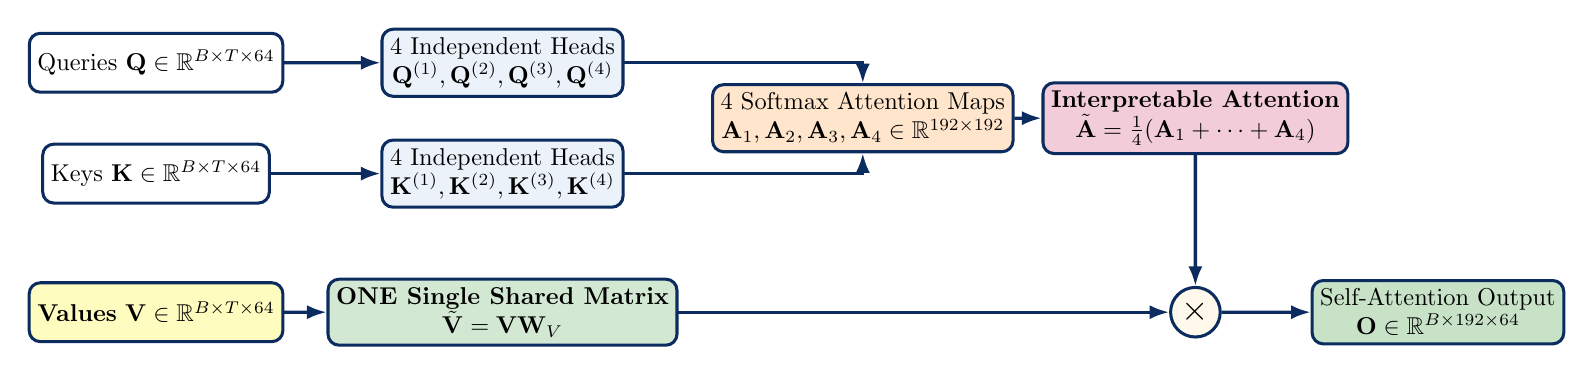
\begin{tikzpicture}[
    scale=0.88, every node/.style={transform shape},
    box/.style={rectangle, draw=navyblue, fill=softblue, rounded corners=4pt, line width=1.1pt, minimum width=2.8cm, minimum height=0.85cm, align=center},
    op/.style={circle, draw=navyblue, fill=softyellow, line width=1.1pt, inner sep=2pt},
    flow/.style={-{Latex[length=2.5mm, width=1.8mm]}, line width=1.2pt, color=navyblue}
]

% Inputs
\node[box, fill=white] (q) at (0, 2.0) {Queries $\mathbf{Q} \in \mathbb{R}^{B \times T \times 64}$};
\node[box, fill=white] (k) at (0, 0.4) {Keys $\mathbf{K} \in \mathbb{R}^{B \times T \times 64}$};
\node[box, fill=yellow!25] (v) at (0, -1.6) {\textbf{Values} $\mathbf{V} \in \mathbb{R}^{B \times T \times 64}$};

% Projections
\node[box] (q_proj) at (5.0, 2.0) {4 Independent Heads\\$\mathbf{Q}^{(1)}, \mathbf{Q}^{(2)}, \mathbf{Q}^{(3)}, \mathbf{Q}^{(4)}$};
\node[box] (k_proj) at (5.0, 0.4) {4 Independent Heads\\$\mathbf{K}^{(1)}, \mathbf{K}^{(2)}, \mathbf{K}^{(3)}, \mathbf{K}^{(4)}$};
\node[box, fill=forestgreen!20] (v_proj) at (5.0, -1.6) {\textbf{ONE Single Shared Matrix}\\$\tilde{\mathbf{V}} = \mathbf{V} \mathbf{W}_V$};

% Softmax Attention
\node[box, fill=orange!20] (scores) at (10.2, 1.2) {4 Softmax Attention Maps\\$\mathbf{A}_1, \mathbf{A}_2, \mathbf{A}_3, \mathbf{A}_4 \in \mathbb{R}^{192 \times 192}$};

% Average
\node[box, fill=purple!20] (avg) at (15.0, 1.2) {\textbf{Interpretable Attention}\\$\tilde{\mathbf{A}} = \frac{1}{4}(\mathbf{A}_1 + \dots + \mathbf{A}_4)$};

% Context
\node[op] (mult) at (15.0, -1.6) {\Large $\times$};
\node[box, fill=forestgreen!25] (out) at (18.5, -1.6) {Self-Attention Output\\$\mathbf{O} \in \mathbb{R}^{B \times 192 \times 64}$};

% Draw
\draw[flow] (q) -- (q_proj);
\draw[flow] (k) -- (k_proj);
\draw[flow] (v) -- (v_proj);

\draw[flow] (q_proj.east) -| (scores.north);
\draw[flow] (k_proj.east) -| (scores.south);

\draw[flow] (scores) -- (avg);
\draw[flow] (avg) -- (mult);
\draw[flow] (v_proj) -- (mult);
\draw[flow] (mult) -- (out);

\end{tikzpicture}%
}
\caption{The Interpretable Multi-Head Self-Attention mechanism. Because all heads share the same $\mathbf{W}_V$ matrix, the four attention maps can be averaged into $\tilde{\mathbf{A}}$, giving a valid percentage attribution across time.}
\label{fig:interpretable_attn}
\end{figure}

\begin{codebox}[Direct Code from \texttt{pipeline/models/tft\_model.py}]
\begin{lstlisting}
class InterpretableMultiHeadAttention(nn.Module):
    def __init__(self, d_model: int, n_heads: int = 4, dropout: float = 0.1):
        super().__init__()
        self.d_model = d_model
        self.n_heads = n_heads
        self.d_head = d_model // n_heads # 64 // 4 = 16

        self.q_proj = nn.Linear(d_model, d_model)
        self.k_proj = nn.Linear(d_model, d_model)
        self.v_proj = nn.Linear(d_model, d_model) # Single shared projection
        self.out_proj = nn.Linear(d_model, d_model)
        self.dropout = nn.Dropout(dropout)

    def forward(self, q: torch.Tensor, k: torch.Tensor, v: torch.Tensor):
        B, T_q, _ = q.shape
        _, T_k, _ = k.shape

        q_proj = self.q_proj(q).view(B, T_q, self.n_heads, self.d_head).transpose(1, 2)
        k_proj = self.k_proj(k).view(B, T_k, self.n_heads, self.d_head).transpose(1, 2)
        v_proj = self.v_proj(v).view(B, T_k, self.n_heads, self.d_head).transpose(1, 2)

        # Dot product: (Q * K^T) / sqrt(d_k)
        scores = torch.matmul(q_proj, k_proj.transpose(-2, -1)) / math.sqrt(self.d_head)
        attn_weights = F.softmax(scores, dim=-1) # (B, n_heads, T_q, T_k)
        attn_weights = self.dropout(attn_weights)

        context = torch.matmul(attn_weights, v_proj) # (B, n_heads, T_q, d_head)
        context = context.transpose(1, 2).contiguous().view(B, T_q, self.d_model)
        output = self.out_proj(context)

        # Average weights across the head dimension for full interpretability
        avg_attn = attn_weights.mean(dim=1) # (B, T_q, T_k)
        return output, avg_attn
\end{lstlisting}
\end{codebox}

---

\section{Quantile Regression and Pinball Loss: Why MSE Fails}

In introductory machine learning courses, almost all regression models are trained using **Mean Squared Error (MSE)**:
\begin{equation}
    \mathcal{L}_{\text{MSE}}(y, \hat{y}) = (y - \hat{y})^2
\end{equation}

\subsection{Why Mean Squared Error is Fatal for Ad Pacing}
\begin{intuitionbox}[The Flaw of the Average]
Mathematically, minimizing $\mathrm{MSE}$ forces the neural network to output the \textbf{conditional mean} $\mathbb{E}[y | x]$.
In a symmetric distribution:
\begin{itemize}
    \item 50\% of actual values will fall \textit{below} the mean.
    \item 50\% of actual values will fall \textit{above} the mean.
\end{itemize}
If your pacing engine allocates budget based on the \textit{mean} expected spend:
\textbf{On half the days of the year, actual spending will exceed your prediction!}
By 2:00 PM or 3:00 PM, the campaign has run completely dry. You cannot protect a multi-thousand dollar budget using the mean. You need an \textbf{upper bound}!
\end{intuitionbox}

\subsection{The Quantile Pinball Loss}
Instead of predicting a single number, TFT predicts three percentiles:
\begin{itemize}
    \item $\hat{y}(0.10)$: The \textbf{10th percentile} (Optimistic / quiet floor). Only 10\% of outcomes fall below this.
    \item $\hat{y}(0.50)$: The \textbf{Median} (The true typical expectation).
    \item $\hat{y}(0.90)$: The \textbf{90th percentile} (Conservative ceiling). There is a 90\% probability that market spend will \textbf{not} exceed this number!
\end{itemize}

How do we train a neural network to predict percentiles instead of means? We use the **Quantile Pinball Loss Function**:
\begin{equation}
    \mathcal{L}_q(y, \hat{y}) = \max\Big( q \cdot (y - \hat{y}), \; (1 - q) \cdot (\hat{y} - y) \Big)
\end{equation}

\begin{figure}[htbp]
\centering
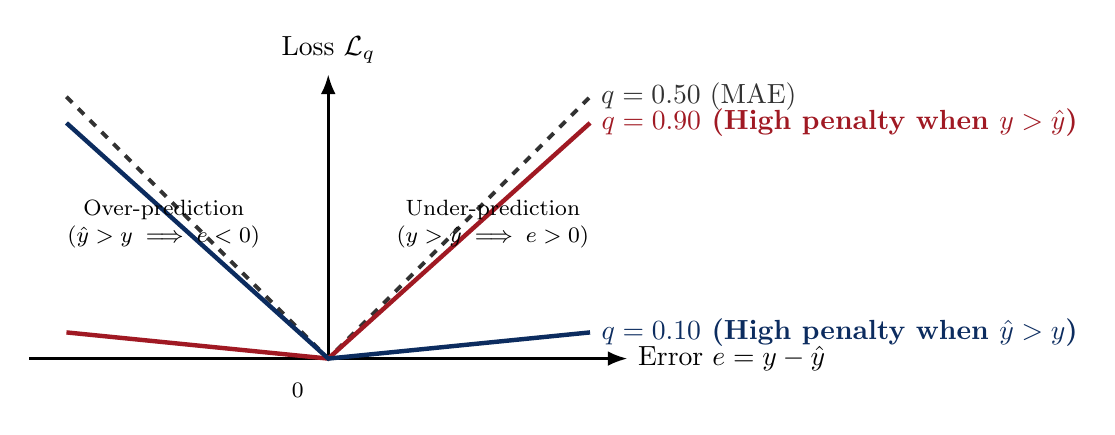
\begin{tikzpicture}[scale=0.95]
    % Axes
    \draw[-{Latex[length=2.5mm]}, line width=1pt] (-4, 0) -- (4, 0) node[right] {Error $e = y - \hat{y}$};
    \draw[-{Latex[length=2.5mm]}, line width=1pt] (0, 0) -- (0, 3.8) node[above] {Loss $\mathcal{L}_q$};
    
    % q = 0.5 (MAE)
    \draw[line width=1.4pt, color=darkgray, dashed] (-3.5, 3.5) -- (0, 0) -- (3.5, 3.5) node[right] {$q = 0.50$ (MAE)};
    
    % q = 0.9 (Heavy penalty for underpredicting)
    \draw[line width=1.6pt, color=crimson] (-3.5, 0.35) -- (0, 0) -- (3.5, 3.15) node[right, font=\bfseries] {$q = 0.90$ (High penalty when $y > \hat{y}$)};
    
    % q = 0.1 (Heavy penalty for overpredicting)
    \draw[line width=1.6pt, color=navyblue] (-3.5, 3.15) -- (0, 0) -- (3.5, 0.35) node[right, font=\bfseries] {$q = 0.10$ (High penalty when $\hat{y} > y$)};

    % Labels
    \node[anchor=north east, font=\footnotesize] at (-0.2, -0.2) {0};
    \node[font=\footnotesize, align=center] at (-2.2, 1.8) {Over-prediction\\($\hat{y} > y \implies e < 0$)};
    \node[font=\footnotesize, align=center] at (2.2, 1.8) {Under-prediction\\($y > \hat{y} \implies e > 0$)};
\end{tikzpicture}
\caption{The Quantile Pinball Loss function for $q=0.10$, $q=0.50$, and $q=0.90$. Notice how $q=0.90$ has a steep slope ($0.9$) when $y > \hat{y}$, forcing the network to predict high enough so it rarely underestimates.}
\label{fig:pinball_loss}
\end{figure}

\begin{mathcheck}[Why Does Pinball Loss Target the $q$-th Quantile? (Calculus Derivation)]
Let us prove why minimizing this loss yields the true $q$-th percentile!
Let $Y$ be a random variable with probability density function $f(y)$ and cumulative distribution function $F(y) = P(Y \le y)$.
We seek the optimal prediction $\hat{y}$ that minimizes expected loss:
\begin{equation}
    \mathbb{E}[\mathcal{L}_q(Y, \hat{y})] = \int_{-\infty}^{\hat{y}} (1 - q)(\hat{y} - y) f(y) \, dy + \int_{\hat{y}}^{\infty} q(y - \hat{y}) f(y) \, dy
\end{equation}
To find the minimum, take the derivative with respect to $\hat{y}$ using the Leibniz Integral Rule:
\begin{align}
    \frac{d}{d\hat{y}}\mathbb{E}[\mathcal{L}_q(Y, \hat{y})] &= (1 - q)\int_{-\infty}^{\hat{y}} f(y) \, dy - q \int_{\hat{y}}^{\infty} f(y) \, dy \\
    &= (1 - q) F(\hat{y}) - q \big(1 - F(\hat{y})\big) \\
    &= F(\hat{y}) - q F(\hat{y}) - q + q F(\hat{y}) \\
    &= F(\hat{y}) - q
\end{align}
Setting the derivative equal to zero to find the critical point:
\begin{equation}
    F(\hat{y}) - q = 0 \implies F(\hat{y}) = q \implies \hat{y} = F^{-1}(q)
\end{equation}
\textbf{The minimizer $\hat{y}$ is precisely the $q$-th quantile of the distribution!}
\end{mathcheck}

\begin{codebox}[Direct Code from \texttt{pipeline/models/tft\_model.py}]
\begin{lstlisting}
def quantile_pinball_loss(y_pred: torch.Tensor, y_true: torch.Tensor, quantiles = [0.10, 0.50, 0.90]) -> torch.Tensor:
    # y_pred shape: (B, horizon, 3)
    # y_true shape: (B, horizon)
    total_loss = 0.0
    for i, q in enumerate(quantiles):
        err = y_true - y_pred[..., i]
        loss_q = torch.maximum(q * err, (q - 1.0) * err)
        total_loss += loss_q.mean()
    return total_loss / len(quantiles)
\end{lstlisting}
\end{codebox}

---

\section{The Closed-Form Pacing Policy \& Budget Solvency Proof}

Now that TFT outputs calibrated 24-hour spending forecasts $\hat{y}_{t+\tau}(0.10)$, $\hat{y}_{t+\tau}(0.50)$, and $\hat{y}_{t+\tau}(0.90)$, how do we convert these numbers into the real-time bid multiplier $\alpha_{t+1}$?

\subsection{The Quantile Throttling Equation}
Let $R_t = B - S_t$ be the remaining budget reserve at hour $t$, where $S_t$ is cumulative spend so far.
The controller updates the bidding multiplier via:
\begin{equation}
    \alpha_{t+1} = \mathrm{clip}\left( \alpha_t \cdot \frac{R_t}{\sum_{\tau=1}^{24} \hat{y}_{t+\tau}(0.90)}, \; 0.05, \; 1.0 \right)
    \label{eq:throttling_rule}
\end{equation}

\begin{intuitionbox}[The Thermostat Analogy]
Look at the ratio inside the equation:
\begin{equation}
    \text{Pacing Ratio} = \frac{\text{Money Remaining in Wallet } (R_t)}{\text{Worst-Case Expected Spend for Next 24 Hours } \left(\sum \hat{y}(0.90)\right)}
\end{equation}
\begin{itemize}
    \item \textbf{Case 1: Money is Abundant ($R_t > \sum \hat{y}(0.90)$):}
    The ratio is $> 1.0$. The campaign has plenty of cash. $\alpha_{t+1}$ increases, bidding more aggressively to capture high-value impressions.
    \item \textbf{Case 2: Money is Tight ($R_t < \sum \hat{y}(0.90)$):}
    The ratio is $< 1.0$. If we keep bidding at rate $\alpha_t$, we will run out of money before the 24-hour horizon ends. The formula automatically scales down $\alpha_{t+1}$, cooling the auction exposure like a thermostat.
\end{itemize}
\end{intuitionbox}

\subsection{Undergraduate Proof of Downside Budget Solvency}
Can we mathematically guarantee that this formula prevents bankruptcy over the 24-hour horizon? Yes!

\begin{theorem}[Downside Budget Solvency]
Assume market clearing spend does not exceed our 90th-percentile conservative forecast:
\begin{equation}
    y_{t+\tau} \le \hat{y}_{t+\tau}(0.90), \quad \forall \tau \in \{1, \dots, 24\}
\end{equation}
Then under update rule~(\ref{eq:throttling_rule}), cumulative spend over the 24-hour horizon is strictly bounded by remaining budget $R_t$:
\begin{equation}
    \sum_{\tau=1}^{24} y_{t+\tau} \le R_t
\end{equation}
\end{theorem}

\begin{proof}
Let us follow the algebra step-by-step:
\begin{enumerate}
    \item In second-price auctions, total expenditure scales monotonically with bid scaling $\alpha$. If the bid multiplier changes from $\alpha_t$ to $\alpha_{t+1}$, realized expenditure scales proportionally:
    \begin{equation}
        Y_{\text{realized}} \le \frac{\alpha_{t+1}}{\alpha_t} \sum_{\tau=1}^{24} \hat{y}_{t+\tau}(0.90)
    \end{equation}
    \item Now substitute our throttling formula for $\alpha_{t+1}$ (in the active unclipped region):
    \begin{equation}
        \alpha_{t+1} = \alpha_t \cdot \frac{R_t}{\sum_{\tau=1}^{24} \hat{y}_{t+\tau}(0.90)}
    \end{equation}
    \item Plug this into the realized spend inequality:
    \begin{align}
        Y_{\text{realized}} &\le \frac{\alpha_t \cdot \frac{R_t}{\sum_{\tau=1}^{24} \hat{y}_{t+\tau}(0.90)}}{\alpha_t} \cdot \left(\sum_{\tau=1}^{24} \hat{y}_{t+\tau}(0.90)\right) \\
        &= \frac{R_t}{\sum_{\tau=1}^{24} \hat{y}_{t+\tau}(0.90)} \cdot \left(\sum_{\tau=1}^{24} \hat{y}_{t+\tau}(0.90)\right) \\
        &= R_t
    \end{align}
    \item The terms cancel out completely! The total spend $Y_{\text{realized}}$ is mathematically bounded by $R_t$.
\end{enumerate}
Therefore, the campaign terminates the horizon with non-negative reserves, guaranteeing budget solvency.
\end{proof}

---

\section{Dual-Boundary Dynamic Spike Detection}

\begin{intuitionbox}[The False Alarm Problem]
Ad traffic is naturally higher at 8:00 PM than at 3:00 AM. If an algorithm sees spend jump from \$20 to \$80 at 8:00 PM, a naive anomaly detector might scream: \textit{``Emergency! Spend jumped 300\%! Slash bids!''}
That would be a mistake. High spend at 8:00 PM is normal circadian traffic. 

We must distinguish between:
\begin{enumerate}
    \item \textbf{Normal predictable diurnal peaks} (handled calmly by TFT).
    \item \textbf{True exogenous market shocks} (e.g., a competitor drops out, causing clearing prices to go crazy).
\end{enumerate}
\end{intuitionbox}

To solve this, our pacing engine implements a **Dual-Boundary Shock Trigger**:
\begin{equation}
    \mathcal{S}_t = \mathbb{I}\Big( y_t > \hat{y}_t(0.90) \Big) \;\land\; \mathbb{I}\left( y_t - \hat{y}_t(0.50) > 1.5 \cdot \frac{B}{T} \right)
\end{equation}

Both conditions must be true simultaneously:
\begin{itemize}
    \item \textbf{Boundary 1 ($y_t > \hat{y}_t(0.90)$):} Realized spend broke above the 90th percentile forecast. This proves the event is statistically improbable.
    \item \textbf{Boundary 2 ($(y_t - \hat{y}_t(0.50)) > 1.5 \frac{B}{T}$):} The deviation from the median is greater than 1.5 times the campaign's nominal hourly velocity. This prevents false alarms during low-budget off-peak hours.
\end{itemize}

When $\mathcal{S}_t = 1$, the pacing engine overrides the normal formula with an emergency brake:
\begin{equation}
    \alpha_{t+1} \leftarrow \min\left(\alpha_{t+1}, \; \alpha_t \cdot \frac{\hat{y}_t(0.50)}{y_t}\right)
\end{equation}
instantly cooling down the bid multiplier before the budget is harmed.

---

\section{Systems Engineering: The Apple Silicon MPS Metal Bug}

When transitioning models from development on x86 Nvidia GPUs to Apple Silicon Macs (M1/M2/M3/M4) using PyTorch Metal Performance Shaders (`mps`), engineers often encounter low-level hardware aborts that never appear in standard textbooks.

\begin{warningbox}[The Mac M4 Abort Trap 6 Error]
When running the initial training script on Apple Silicon MPS:
\begin{verbatim}
MPSCore/Types/MPSNDArray.mm:893: failed assertion 
`[MPSNDArray, initWithBufferImpl:offset:descriptor:isForNDArrayAlias:isUserBuffer:] 
Error: buffer is not large enough. Must be 1376256 bytes'
scripts/train_mac_m4.sh: line 40: 16492 Abort trap: 6
\end{verbatim}
Where did the exact number $1,376,256$ bytes come from, and why did PyTorch crash?
\end{warningbox}

\subsection{Virtual Tensors vs. Physical Memory Buffers}
In PyTorch, suppose you have a static context vector $\mathbf{s} \in \mathbb{R}^{B \times 1 \times d}$ ($B=32$, $d=64$).
You want to broadcast this vector across all $k=168$ hours of lookback:
\begin{lstlisting}
# Standard PyTorch virtual broadcast
context = s.unsqueeze(1).expand(-1, 168, -1) # Shape: (32, 168, 64)
\end{lstlisting}

What happens in computer RAM when you call `.expand()`?
\begin{itemize}
    \item PyTorch uses a clever trick called **Stride-0 Virtual Broadcasting**.
    \item It \textbf{does not copy the data 168 times}. Instead, it keeps a single row in memory and sets the memory stride along dimension 1 to $0$:
    \begin{equation}
        \text{Physical Bytes Allocated} = 32 \times 1 \times 64 \times 4\text{ bytes (float32)} = \mathbf{8,192\text{ bytes}}
    \end{equation}
    \item When PyTorch reads time step 0, 1, or 167, it simply loops back to the same 8 KB memory address.
\end{itemize}

\begin{figure}[htbp]
\centering
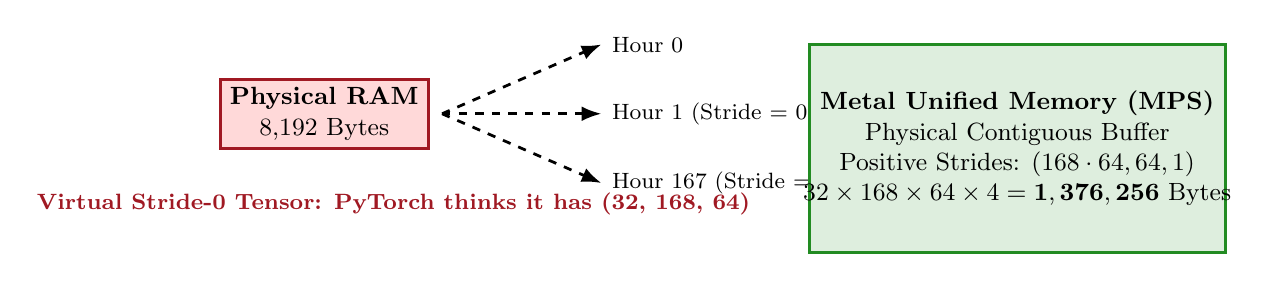
\begin{tikzpicture}[scale=0.88]
    % Virtual stride-0
    \draw[fill=red!15, draw=crimson, line width=1.1pt] (0, 2) rectangle (3, 3);
    \node[align=center, font=\small] at (1.5, 2.5) {\textbf{Physical RAM}\\8,192 Bytes};
    
    \draw[-{Latex[length=2.5mm]}, line width=1pt, dashed] (3.2, 2.5) -- (5.5, 3.5) node[right, font=\footnotesize] {Hour 0};
    \draw[-{Latex[length=2.5mm]}, line width=1pt, dashed] (3.2, 2.5) -- (5.5, 2.5) node[right, font=\footnotesize] {Hour 1 (Stride = 0)};
    \draw[-{Latex[length=2.5mm]}, line width=1pt, dashed] (3.2, 2.5) -- (5.5, 1.5) node[right, font=\footnotesize] {Hour 167 (Stride = 0)};
    
    \node[font=\footnotesize\bfseries, color=crimson] at (2.5, 1.2) {Virtual Stride-0 Tensor: PyTorch thinks it has (32, 168, 64)};

    % Physical MPS
    \draw[fill=forestgreen!15, draw=forestgreen, line width=1.1pt] (8.5, 0.5) rectangle (14.5, 3.5);
    \node[align=center, font=\small] at (11.5, 2.0) {\textbf{Metal Unified Memory (MPS)}\\Physical Contiguous Buffer\\Positive Strides: $(168 \cdot 64, 64, 1)$\\$32 \times 168 \times 64 \times 4 = \mathbf{1,376,256\text{ Bytes}}$};
\end{tikzpicture}
\caption{Comparison of PyTorch virtual stride-0 broadcasting (left) versus Apple Silicon Metal Performance Shaders physical buffer requirements (right).}
\label{fig:mps_buffer}
\end{figure}

\subsection{Why Metal Performance Shaders (MPS) Crashed}
On Apple Silicon, PyTorch offloads matrix multiplications to Apple's Metal graphics/neural framework via `MPSNDArray`.
Metal kernels do not support arbitrary stride-0 pointers in dense matrix multiplication routines.
Before running the kernel, the Metal driver checks the tensor descriptor:
\begin{align}
    \text{Required Memory} &= \text{Batch} \times \text{Time} \times \text{Channels} \times \text{BytesPerFloat} \\
    &= 32 \times 168 \times 64 \times 4\text{ bytes} = \mathbf{1,376,256\text{ bytes}}
\end{align}
Metal inspected the actual allocated pointer:
\begin{equation}
    \text{Actual Memory Allocated} = 8,192\text{ bytes}
\end{equation}
Because $8,192 < 1,376,256$, Metal triggered a hardware assertion failure to prevent a catastrophic segmentation fault or memory corruption!

\subsection{The Architectural Solution}
To guarantee flawless execution on Apple Silicon Mac M4 chips, we replaced virtual `.expand()` with physical `.repeat().contiguous()`:
\begin{lstlisting}
# FIXED: Physically allocate genuine memory buffer for Apple Silicon MPS
context_past = static_context.unsqueeze(1).repeat(1, self.lookback, 1).contiguous()
\end{lstlisting}
Calling `.repeat(1, 168, 1)` physically duplicates the memory in unified RAM, creating a genuine $1,376,256$-byte buffer with positive memory strides. Metal verification succeeds immediately!

---

\section{Summary: End-to-End Mathematical Tensor Roadmap}

Table~\ref{tab:complete_summary} presents the complete summary of every mathematical operation in the TFT ad pacing model, from the raw input features to the final bidding multiplier.

\begin{table}[htbp]
\centering
\caption{Consolidated Architectural Pipeline of the TFT Pacing Model}
\label{tab:complete_summary}
\small
\begin{tabular}{llll}
\toprule
\textbf{Pipeline Stage} & \textbf{Mathematical Operation} & \textbf{Tensor Shape} & \textbf{Physical Meaning} \\
\midrule
1. Static Linear & $\tilde{\mathbf{s}}_j = \mathbf{W}_{s,j} s_j + \mathbf{b}_{s,j}$ & $(32, 3, 16)$ & Embeds budget and duration \\
2. Static VSN & $\mathbf{c}_s = \sum v_j \mathrm{GRN}(\tilde{\mathbf{s}}_j)$ & $(32, 64)$ & Campaign context vector \\
3. Past Observed & $\tilde{\mathbf{z}} = \mathrm{VSN}_{\text{past}}(\mathbf{z}_t, \mathbf{c}_s)$ & $(32, 168, 64)$ & Noise-filtered 7-day spend \\
4. Future Known & $\tilde{\mathbf{x}} = \mathrm{VSN}_{\text{future}}(\mathbf{x}_t, \mathbf{c}_s)$ & $(32, 24, 64)$ & Filtered circadian features \\
5. Timeline Concat & $\tilde{\mathbf{\Xi}} = [\tilde{\mathbf{z}}, \; \tilde{\mathbf{x}}]$ & $(32, 192, 64)$ & 8-day unified horizon \\
6. Static Enrich & $\mathbf{\Xi}_e = \mathrm{GRN}(\tilde{\mathbf{\Xi}}, \mathbf{c}_s)$ & $(32, 192, 64)$ & Injects budget into timeline \\
7. LSTM Seq2Seq & $\mathbf{H}_{\text{lstm}} = \mathrm{LSTM}(\mathbf{\Xi}_e)$ & $(32, 192, 64)$ & Local step-to-step smoothing \\
8. Self-Attention & $\mathbf{H}_{\text{attn}} = \tilde{\mathbf{A}}(\mathbf{Q}, \mathbf{K}) (\mathbf{V}\mathbf{W}_V)$ & $(32, 192, 64)$ & Interpretable weekly search \\
9. Quantile Head & $\hat{\mathbf{y}} = \mathbf{W}_{\text{out}} \mathbf{H}_{\text{attn}}[:, 168:, :]$ & $(32, 24, 3)$ & Outputs $q \in \{0.10, 0.50, 0.90\}$ \\
10. Pinball Loss & $\mathcal{L}_q = \max(q e, (q-1)e)$ & Scalar & Calibrated quantile training \\
11. Pacing Policy & $\alpha_{t+1} = \alpha_t \frac{R_t}{\sum \hat{y}(0.90)}$ & Scalar & Downside solvency bound \\
12. Shock Trigger & $\mathcal{S}_t = \mathbb{I}(y > \hat{y}_{90}) \land \mathbb{I}(\Delta y > 1.5 \frac{B}{T})$ & Binary & Dual-boundary spike brake \\
\bottomrule
\end{tabular}
\end{table}

\section{Conclusion}
By decomposing the Temporal Fusion Transformer into its elementary linear algebra and calculus components, we see that it is not magic:
\begin{enumerate}
    \item \textbf{GLUs} act as soft electronic switches to suppress irrelevant paths.
    \item \textbf{GRNs} allow deep networks to safely bypass layers when data is already clean.
    \item \textbf{VSNs} assign real-time percentage weights to filter out erratic auction jitter.
    \item \textbf{Shared-Value Attention} allows multi-head models to provide genuine percentage interpretability.
    \item \textbf{Quantile Pinball Loss} prevents premature budget bankruptcy by predicting conservative 90th-percentile ceilings.
    \item \textbf{Physical Buffer Contiguity} ensures compatibility with high-performance Apple Silicon Metal hardware.
\end{enumerate}
With this architectural foundation, the pacing engine successfully prevents premature budget depletion while delivering smooth, optimal ad spend across real-time programmatic auctions.

\end{document}
